\textcolor{red}{Introduzione ...}

\section{Architettura e tecnologie utilizzate}

\textcolor{red}{Introduzione ...}

\subsection{Backend\label{sec:architettura-backend}}

In questa sezione si vuole analizzare nel dettaglio l'architettura messa a punto per il backend di CAMUS, specificando le motivazioni che hanno portato alla sua realizzazione, e la descrizione delle tecnologie che hanno permesso lo sviluppo della soluzione.

\begin{figure}[ht]
	\centering
	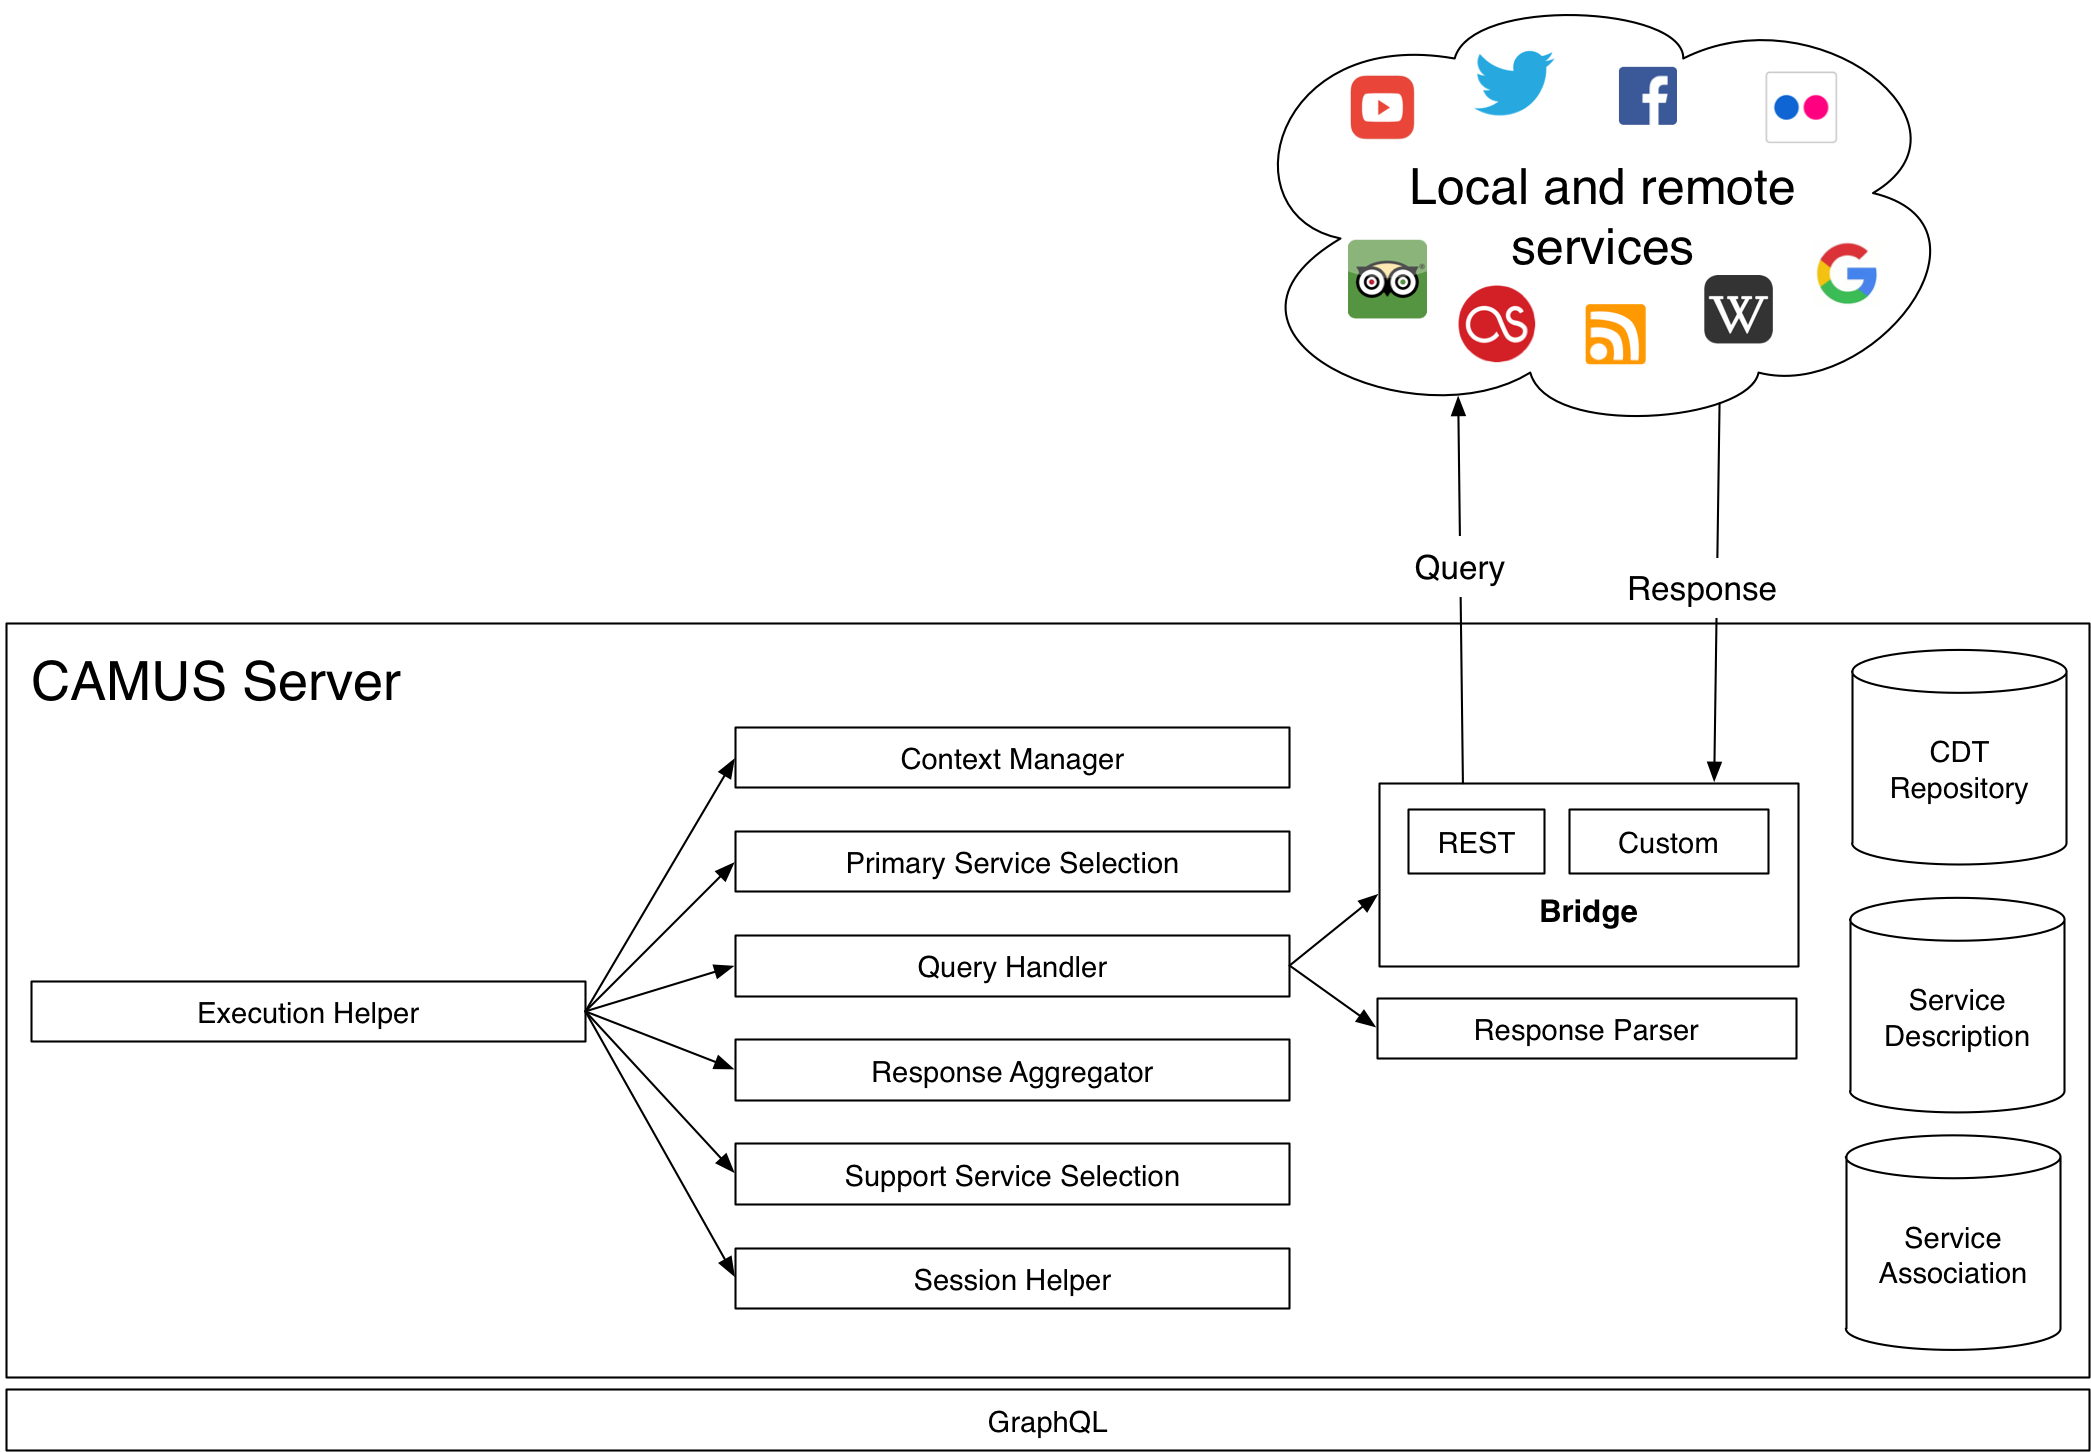
\includegraphics[width=\textwidth]{4-progettazione-alto-livello/Immagini/camus-architecture-backend.png}
	\caption{Architettura del backend}\label{fig:architettura-backend}
\end{figure}

L'architettura di CAMUS viene descritta schematicamente in Figura \ref{fig:architettura-backend}. Come si può notare è stata privilegiata la modularità dei vari componenti che formano il sistema, in modo che il compito di ognuno fosse ben circoscritto. Inoltre tutti i componenti mostrati sono \emph{stateless}, cioè non mantengono informazioni sullo stato di una sessione. Questa scelta architetturale permette di poter avviare diverse istanze del backend di CAMUS per poter soddisfare le molteplici richieste degli utenti. Questa scelta permette di selezionare quale nodo sia il miglior candidato per gestire una richiesta in coda in base a politiche che non riguardano lo stato della sessione (es.: disponibilità del nodo, basso carico sul sistema, ecc.).

Il componente che coordina tutti gli altri è l'\emph{Execution Helper}. Il suo compito è quello di inizializzare tutti gli altri componenti e organizzare le chiamate secondo il flusso della richiesta (che verrà analizzato nel dettaglio nella Sezione \ref{sec:flusso-richiesta-server}).

Il \emph{Context Manager} è il componente che si occupa di ricevere il contesto inviato dalla mobile app e trasformarlo in una versione \virgolette{decorata}, eseguendo un'unione tra le informazioni ricevute dal client e quelle del descrittore completo del CDT. In questo modo viene agevolata l'esecuzione dei componenti successivi, in quanto le informazioni necessarie all'elaborazione sono già state catalogate e definite in modo corretto.

Il compito del \emph{Primary Service Selection} è di andare a recuperare le associazioni tra l'albero di contesto e le operazioni dei servizi primari. \upe inoltre suo compito gestire le associazioni personalizzate, come quella relativa alla ricerca tramite \emph{località}. In seguito assegna un \emph{punteggio} a ogni operazione identificata ed emette in uscita le prime N operazioni con valutazione più elevata.

Un compito simile viene svolto dal \emph{Support Service Selection} per le operazioni di supporto. Sebbene lo scopo del componente sia lo stesso l'algoritmo di selezione è differente: in questo caso viene effettuato un \emph{conteggio} del numero di associazioni trovate e successivamente si verifica che soddisfi il minimo numero di associazioni.

Il \emph{Query Handler} ha il compito di gestire le chiamate verso i servizi. Acquisisce la lista di operazioni scelte dal \emph{Primary Service Selection} e ne recupera i \emph{descrittori}, contenenti le informazioni per poterli interrogare. Successivamente organizza le chiamate ai servizi attraverso l'uso di \emph{bridge} specifici, scelti in base al \emph{protocollo} di comunicazione adottato dal servizio. Una volta ricevute le risposte, si occupa di interfacciarsi con il \emph{Response Parser} per trasformarle nella rappresentazione interna, che sfrutta dei \emph{termini semantici} come nome dei campi.

Infine il \emph{Response Aggregator} ha il compito di analizzare gli elementi ricevuti al fine di rimuovere i duplicati.

Il \emph{Session Helper} si occupa di gestire le richieste verso pagine successive alla prima, in quanto richiede una fase di preparazione aggiuntiva. Il componente analizza lo stato della richiesta e smista i dati quando sono disponibili altrimenti effettua nuove richieste verso i servizi per acquisire ulteriori informazioni.

Per quanto riguarda l'esposizione dei metodi che possono essere richiamati dal client si è deciso di non utilizzare un approccio basato sull'esposizione di endpoint REST bensì di sperimentare GraphQL.

In questa sezione si è voluta dare una visione d'insieme sui compiti che spettano ai vari componenti. Un'analisi più approfondita delle attività di ognuno di essi verrà svolta nella Sezione \ref{sec:componenti-backend}.

Ora che è stata presentata l'architettura si procede con la descrizione delle tecnologie che hanno permesso la realizzazione del backend. Una panoramica è già stata fornita nella Sezione \ref{sec:tecnologie-backend-background} mentre di seguito si vogliono descrivere quali sono i moduli specifici utilizzati per sviluppare alcune parti del sistema e per far comunicare i vari componenti.

Per gestire le funzionalità del server viene utilizzato il web framework \emph{ExpressJS}\footnote{ExpressJS: \url{http://expressjs.com/}}. \emph{ExpressJS} è un framework molto leggero, che mette a disposizione le funzionalità base affinché un server sia operativo. Ha la potenzialità di avere un ottimo sistema di \emph{middleware}, che permette di utilizzare altre funzionalità più avanzate.

Per \emph{GraphQL} viene utilizzata l'implementazione specifica per Javascript rilasciata da Facebook\footnote{GraphQL-js: \url{https://github.com/graphql/graphql-js}} e l'estensione di \emph{Relay}\footnote{Relay-GraphQL: \url{https://github.com/graphql/graphql-relay-js}} per gestire le connessioni. Affinché gli schemi di \emph{GraphQL} possano essere esposti dal server si sfrutta l'apposito middleware \emph{Express-GraphQL}\footnote{Express-GraphQL: \url{https://github.com/graphql/express-graphql}}.

MongoDB non possiede una struttura dello schema del database definita a priori. Per garantire coerenza coi dati memorizzati si è scelto di utilizzare un Object Relational Mapping (ORM)\footnote{Object Relational Mapping: \url{https://it.wikipedia.org/wiki/Object-relational_mapping}}. Un ORM fornisce un livello di astrazione superiore a un driver nativo e permette di specificare come gli oggetti vengono mappati nel database e viceversa, definendo implicitamente uno schema del database. In particolare, per il progetto CAMUS è stato utilizzato un ORM specifico per Node.js di nome \emph{mongoose}\footnote{MongooseJS: \url{http://mongoosejs.com/}}.

Infine, per interfacciare Node.js con l'istanza di Redis in esecuzione viene utilizzato il modulo \emph{ioredis}\footnote{ioredis: \url{https://github.com/luin/ioredis}}.

\subsection {Mobile app}\label{sec:architettura-applicazione}

\begin{figure}[h]
	\centering
	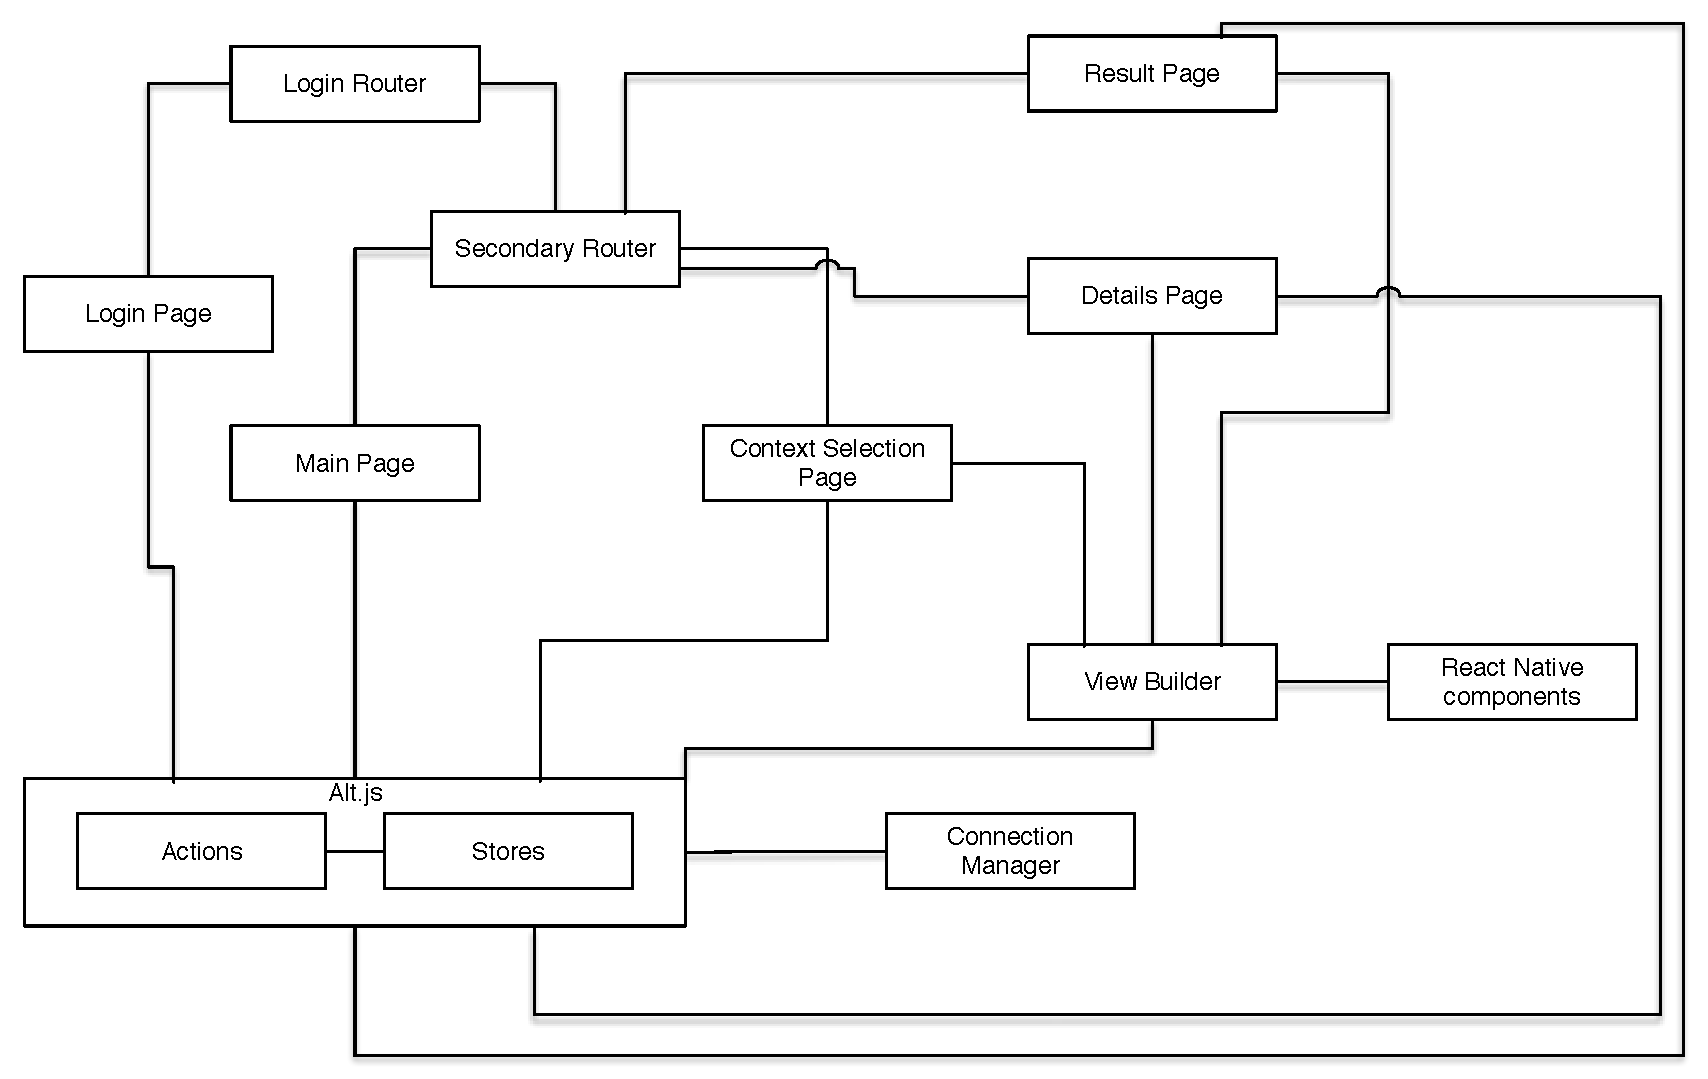
\includegraphics[width=\textwidth]{4-progettazione-alto-livello/Immagini/app_architecture.pdf}
	\caption{Architetture generale dell'app CAMUS}\label{fig:app-architecture}
\end{figure}

E’ possibile osservare l’architettura dell’app CAMUS in Figura \ref{fig:app-architecture}. Per una migliore comprensione dello schema nelle sezioni seguenti verranno analizzati nel dettaglio i singoli componenti che la compongono.

\subsubsection{Pagine dell'applicazione}

Essendo un progetto basato su JavaScript per poter controllare le diverse pagine dell'applicazione è necessario utilizzare un \emph{router}. Si è scelto di sfruttare due \emph{router} diversi, uno per gestire il \emph{login} e un altro per la navigazione all'interno dell'applicazione. Il \emph{router} per il \emph{login} controlla solamente se l'utente è loggato e ha lo scopo di non permettere l'accesso alle pagine che necessitano di autenticazione. Come percorsi possiede \emph{Login Page} e il \emph{secondary router}, che racchiude la navigazione effettiva dell'utente autenticato.

\begin{figure}[H]
	\centering
	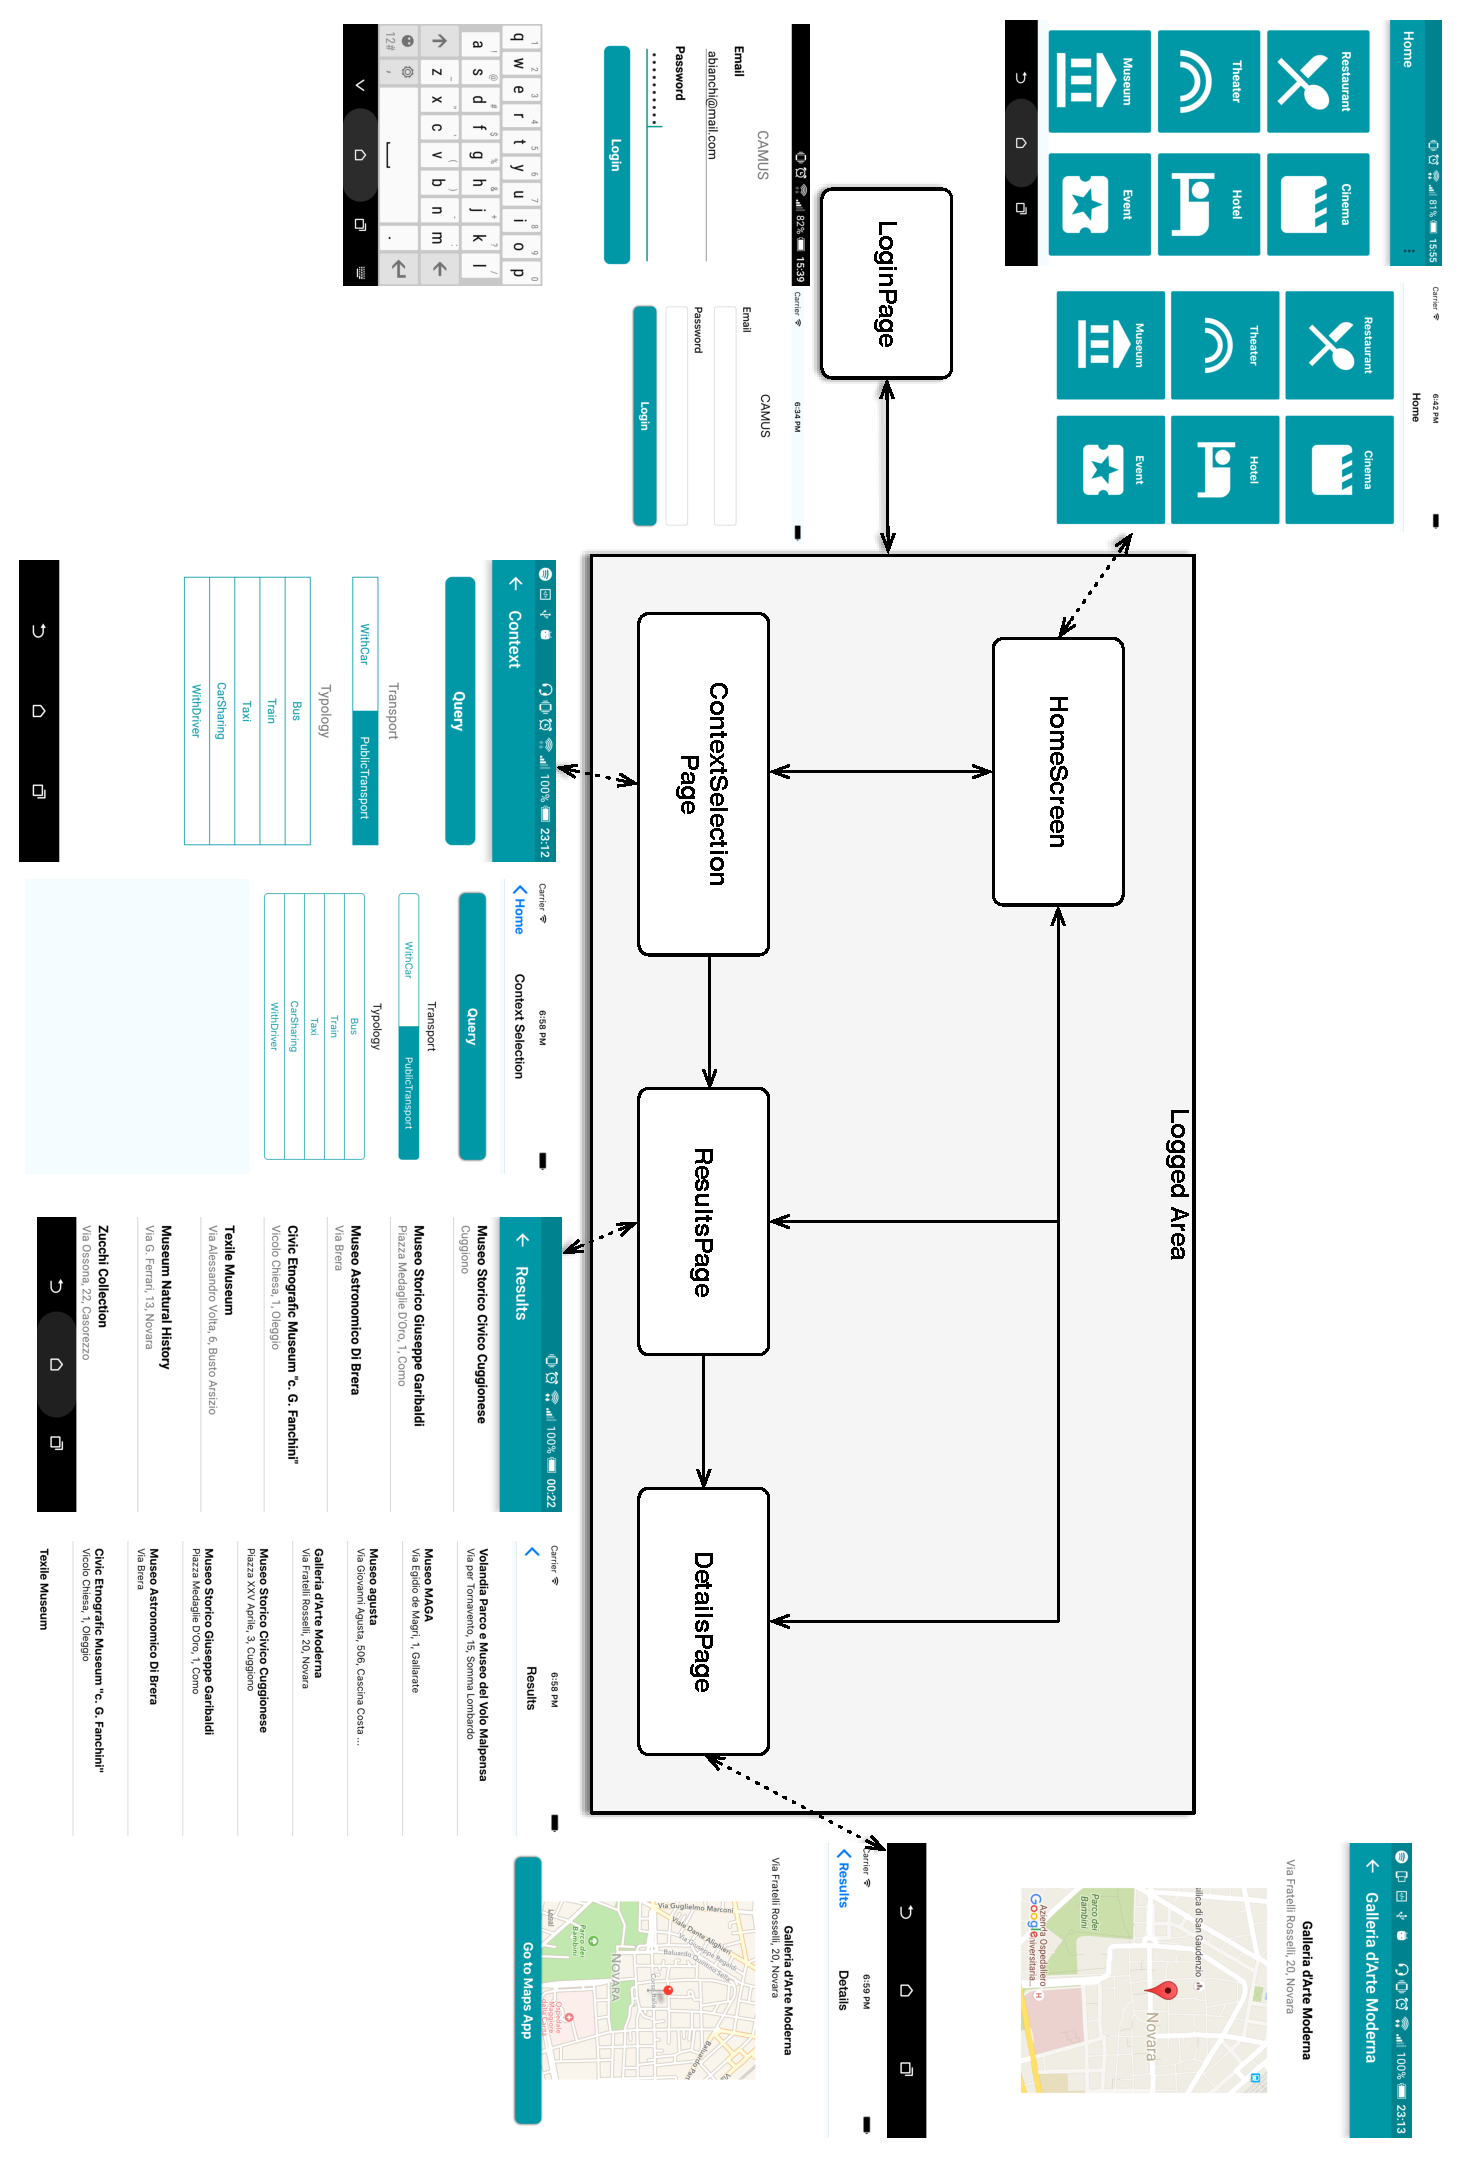
\includegraphics[width=\textwidth]{4-progettazione-alto-livello/Immagini/screen_schema.pdf}
	\caption{Schema delle pagine}\label{fig:screen-schema}
\end{figure}

Come si può notare nella Figura \ref{fig:screen-schema}, le pagine sono le seguenti:

\begin{itemize}
	\item \textbf{Login Page}
	\upe la pagina dove l'utente inserisce le proprie credenziali per accedere al sistema CAMUS e ottenere i parametri per il corretto funzionamento dell'applicazione
	\item \textbf{Logged Area}
	Si tratta della parte dell'applicazione alla quale l'utente può accedere nel caso in cui sia autenticato e gestisce le pagine di selezione del contesto e di visualizzazione dati:
	\begin{itemize}
		\item \textbf{Main Page}
		È la pagina principale dell'applicazione e permette all'utente di mostrare tutti gli \emph{Interest Topic} presenti nel suo CDT. La scelta della categoria desiderata permette di accedere alla \emph{Context Selection Page}
		\item \textbf{Context Dimension Page}
		In questa pagina viene chiesto il contesto all'utente mediante un'interfaccia che si adatta a runtime man mano che l'utente effettua delle scelte per guidarlo nella definizione del contesto da inviare come richiesta al server. Una volta composto il contesto viene costruita la query e inviata all'endpoint GraphQL del server CAMUS. 
		\item \textbf{Results Page}
		Si tratta della pagina che deve mostrare l'intero dataset proveniente dal server e gestisce la paginazione dei risultati, a seconda della posizione del cursore dell'utente nella ListView 
		\item \textbf{Details Page}
		In questa pagina vengono visualizzati i dettagli dell'oggetto selezionato e sono gestiti i collegamenti con le applicazioni esterne, per mezzo della libreria di \emph{Linking} di React Native o tramite moduli personalizzati
	\end{itemize}
\end{itemize}

\subsubsection{Helpers}

Le pagine descritte nella sezione precedente utilizzano alcuni componenti che sono in comune tra tutte le pagine dell'applicazione in quanto aiutano a eseguire funzionalità comuni. Di seguito sono elencati i componenti che svolgono questo compito:

\begin{itemize}
	\item \textbf{Connection Manager}
	In questo componente vengono gestite tutte le connessioni con l'\emph{endpoint} GraphQL. Permette di gestire la fase di login e di scambio dati per scaricare il CDT, gli schemi di mashup e i dati. Per quanto riguarda i dati sono esposti due metodi distinti, il primo per gestire la prima richiesta di nuovi dati, il secondo per quelle successive, chiedendo una nuova pagina come spiegato nella Sezione \ref{sec:paginazione-app}
	\item \textbf{View Builder}
	Si tratta del componente che costruisce le \emph{view} dinamiche partendo dallo schema di mashup, scaricato assieme al CDT appena effettuato il \emph{login}	
	\item \textbf{StyleSheet}
	Si tratta del foglio di stile nel quale sono impostati tutti i parametri predefiniti per la visualizzazione dei componenti dell'applicazione
\end{itemize}

\subsubsection{Actions\label{sec:actions}}

Le \emph{Actions} sono i metodi invocati dall'ap\-pli\-ca\-zio\-ne per modificare lo stato dell'ap\-pli\-ca\-zio\-ne. Nell'applicazione CAMUS sono utilizzate principalmente in due modi:

\begin{itemize}
	\item \textbf{Data Fetching}
	Quando è necessario scaricare gli elementi necessari per il corretto funzionamento dell'applicazione (CDT e mashup) o i dati provenienti dalle richieste, le action hanno lo scopo di modificare lo stato per cambiare la view dell'applicazione a seconda dello stato della richiesta.
	Per esempio quando si preme il bottone per effettuare una nuova richiesta basata sul contesto viene invocata un'azione per mantenere lo stato coerente tra più componenti e permettere di mostrare in fase di caricamento uno Spinner e una volta che i dati sono arrivati all'interno dell'applicazione mostrarli nella ListView
	\item \textbf{Application State}
	Lo stato generale dell'applicazione viene salvato utilizzando delle \emph{Action} chiamate dalle interazioni dell'utente con l'interfaccia grafica. Per esempio quando viene composto il contesto le diverse selezioni sono passate dall'utente tramite le Action nelle Store
\end{itemize}	

Le \emph{Actions} che sono state implementate nell'applicazione sono le seguenti:

\begin{itemize}
	\item \textbf{User Actions}
	Sono le azioni che servono ad aggiornare i parametri relativi all'utente, come password, email e suo identificativo nel database:
	\begin{itemize}
		\item \textbf{Update Email}
		Metodo per aggiornare l'email dell'utente 
		\item \textbf{Update Password}
		Metodo per aggiornare la password dell'utente
		\item \textbf{Update Token}
		Metodo per tenere in memoria il Token della connessione col server per ottenere il CDT
	\end{itemize}
	\item \textbf{Context Actions}
	Sono le azioni che gestiscono la selezione del contesto, consentendo di modificare le scelte effettuate dall'utente:
	\begin{itemize}
		\item \textbf{Set Transport}
		Metodo per salvare la tipologia di trasporto da parte dell'utente
		\item \textbf{Set Typology}
		Metodo per salvare la tipologia nel caso di trasporto non con mezzi propri
		\item \textbf{Add Forbidden}
		Metodo per aggiungere un parametro in quelli da nascondere all'utente
		\item \textbf{Remove Forbidden}
		Metodo per rimuovere il parametro selezionato dalla lista di quelli da nascondere all'utente
		\item \textbf{Update Last Context}
		Metodo per salvare l'ultimo contesto inviato al server, per poterlo riutilizzare nelle richieste per le pagine successive
	\end{itemize}
	\item \textbf{View Actions}
	Sono le azioni relative alla gestione dei mashup ma non dello stato della navigazione, per le quali è utilizzato un componente aggiuntivo sempre basato su Flux (React Native Router Flux):
	\begin{itemize}
		\item \textbf{Set Views}
		Metodo per salvare il file con le view provenienti dal server 
		\item \textbf{Select Interest Topic}
		Metodo per salvare l'\emph{Interest Topic} corrente selezionato da parte dell'utente
	\end{itemize}
	\item \textbf{Data Actions}
	Trattano della gestione del CDT e dei risultati ottenuti dal server:
	\begin{itemize}
		\item \textbf{Update Results}
		Metodo per aggiornare i dati dei risultati provenienti dalla query basata sul contesto
		\item \textbf{Results Failed}
		Metodo per inviare il messaggio di errore proveniente dalla richiesta
		\item \textbf{Update Full CDT}
		Metodo per aggiornare il CDT associato all'utente
	\end{itemize}
\end{itemize}

\subsubsection{Stores\label{sec:action-store}}

Le \emph{Stores} salvano lo stato dell'applicazione viene salvato e forniscono alle view nuovi dati ogni volta che sono aggiornate. 
Per ogni interazione sui dati dell'applicazione che necessitano di rimanere persistenti viene invocata una action dal componente e dalla view che si propaga prima nelle store, e successivamente aggiorna nuovamente la view.
Si è scelto di suddividere le \emph{Store} per tipologia di operazione e dato trattata:

\begin{itemize}
	\item  \textbf{User Store}
	Nella \emph{User Store} sono memorizzati tutti i dati relativi all'utente. In particolare viene memorizzata la mail dell'utente nel database del server e l'identificativo del CDT a lui associato, che serviranno per poter effettuare le query GraphQL per ottenere i dati
	\item \textbf{Context Store}
	Nel \emph{Context Store} vengono gestiti i dati che riguardano i dati di contesto, come le coordinate geografiche e le scelte delle tipologie di trasporto pubblico, in modo da essere riutilizzate. Per quanto riguarda le richieste di dati, una volta che il contesto viene composto per effettuare la prima query, questo payload viene salvato qui e poi riutilizzato nelle query dei risultati successivi
	\item \textbf{View Store}
	In questa store sono memorizzati tutti i dati relativi alle view. Qui viene salvato lo schema di mashup e l'\emph{Interest Topic} corrente
	\item \textbf{Data Store}
	Si tratta della store più complessa perchè deve gestire in modo dinamico diverse tipologie di dato. Quando viene ricevuto il CDT vengono scanditi gli \emph{interest topic} è creato un oggetto nel campo \emph{results} che è composto da un array di tanti oggetti definiti da due campi:
	\begin{enumerate}
		\item \textbf{Results}
		Rappresenta i risultati ricevuti per quell'\emph{interest topic}, comprende i dai servizi primari e i collegamenti per i servizi di supporto
		\item \textbf{Topic}
		Rappresenta l'\emph{Interest topic} associato ai risultati ricevuti dal server
	\end{enumerate}
	Questa operazione è necessaria per poter gestire il fatto di avere comunque dei dati in memoria in condizioni di assenza di rete, anche per tipi diversi di risultati provenienti dal server e per essere in grado di gestire una cardinalità variabile di tipologie di dati. Nel Listato \ref{lst:store-two-topics} è mostrato come viene rappresentato lo stato nel caso in cui l'utente abbia a disposizione due \emph{Interest Topic} e la suddivisione dei risultati per le due tipologie, in questo caso \emph{Restaurants} ed \emph{Event}. Si noti che oltre ai risultati sono salvati anche i parametri con lo stato della paginazione, per lasciare la possibilità di riprendere la visione di nuovi risultati.
\end{itemize}

\begin{listing}[H]
	\inputminted{json}{4-progettazione-alto-livello/Codice/store-two-topics.json}
	\caption{Esempio Data Store Mashup}
	\label{lst:store-two-topics}
\end{listing}

\section{Flusso di una richiesta}

\subsection{Backend\label{sec:flusso-richiesta-server}}

In questa sezione viene analizzato il flusso di esecuzione principale del sistema, quello che riguarda le richieste proveniente dalla mobile app. Le prime attività che svolge sono il login dell'utente, tramite l'endpoint \emph{login} (Sezione \ref{sec:login-endpoint}), e l'acquisizione dei dati personali dell'utente, tramite l'endpoint \emph{getPersonalData} (Sezione \ref{sec:get-personal-data-endpoint}).

L'attività più importante riguarda invece l'endpoint \emph{executeQuery} (Sezione \ref{sec:execute-query-endpoint}), che è dedicato all'invio delle informazioni trovate in base al contesto dell'utente. In Figura \ref{fig:flusso-nuova-richiesta} vengono mostrati i componenti coinvolti in questa fase e l'ordine col quale sono eseguiti.

\begin{figure}[ht]
	\centering
	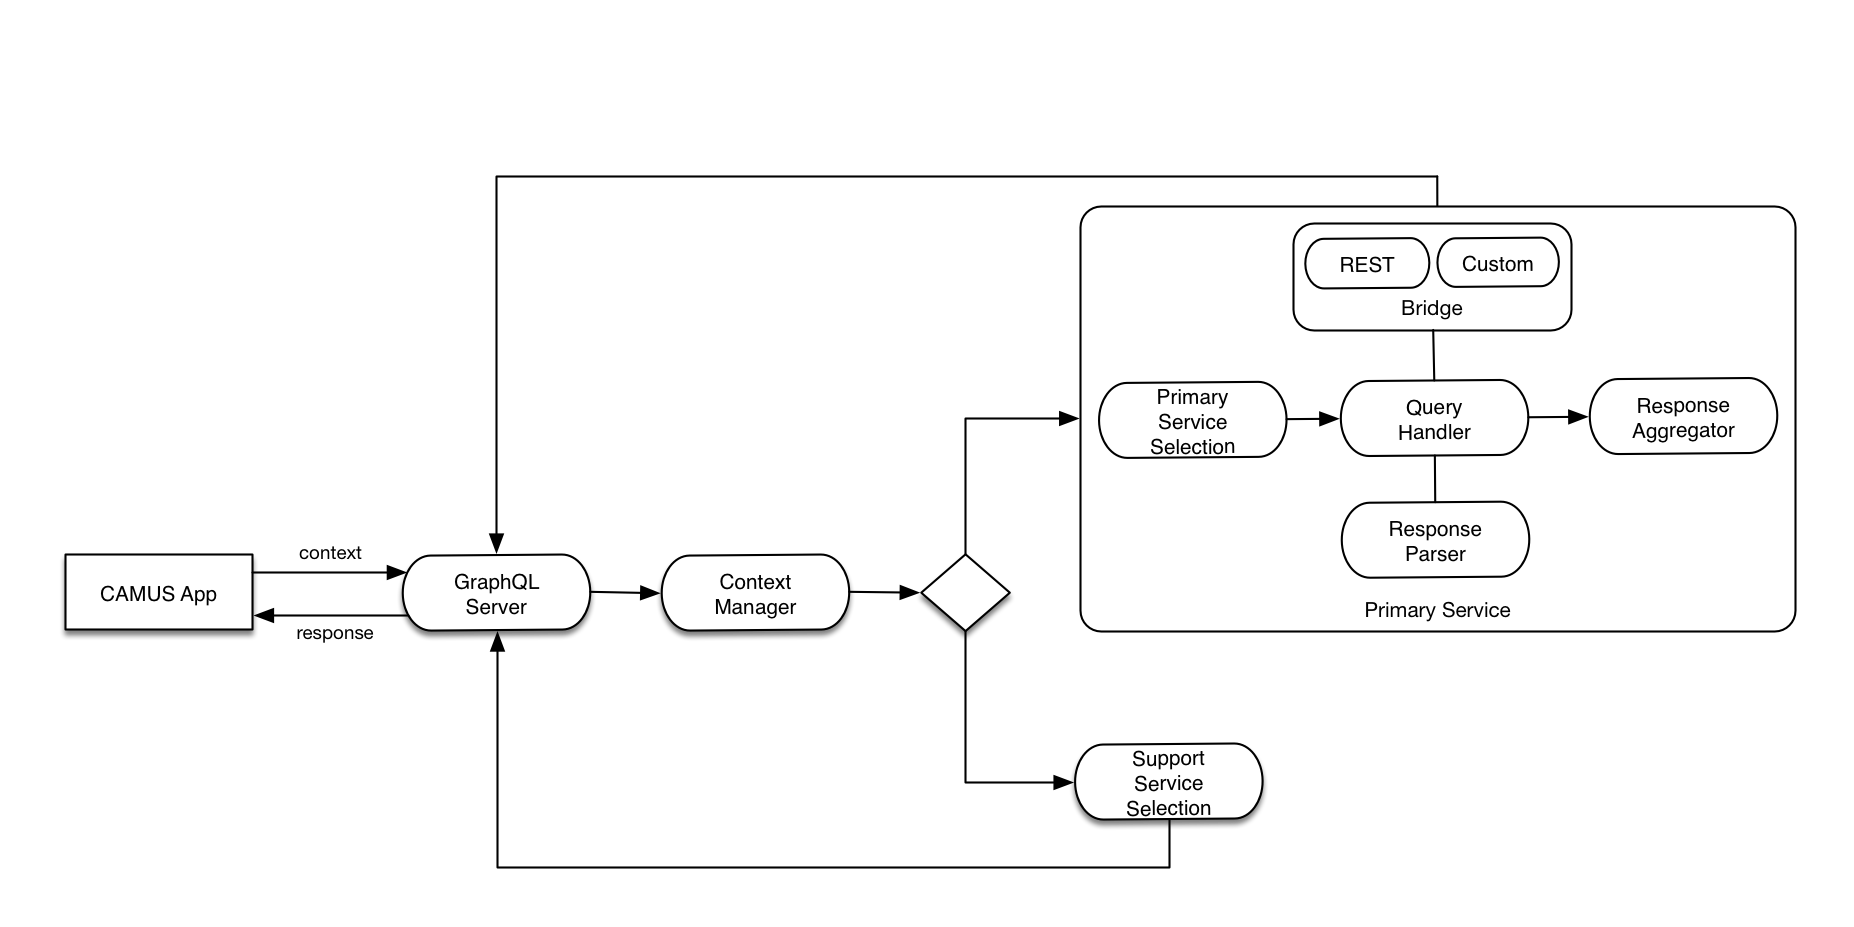
\includegraphics[width=\textwidth]{4-progettazione-alto-livello/Immagini/flusso-richiesta-backend.png}
	\caption{Flusso di una nuova richiesta\label{fig:flusso-nuova-richiesta}}
\end{figure}

L'attività viene divisa in tre fasi:

\begin{enumerate}
	\item \textbf{Creazione CDT decorato}
	\upe la prima fase che viene eseguita. Una volta ricevuto il \emph{contesto} dal client, questo viene analizzato e trasformato nella versione \emph{decorata}
	\item \textbf{Acquisizione dati primari}
	Questa fase avviene dopo la creazione del CDT decorato. Si occupa di selezionare le operazioni attinenti al contesto, interrogare i servizi, integrare le risposte e inviare i dati finali al client
	\item \textbf{Composizione servizi di supporto}
	Questa fase avviene dopo la creazione del CDT e in parallelo all'acquisizione dei dati primari. A partire dal contesto si occupa di selezionare i servizi di supporto richiesti dal client e ne compone le query
\end{enumerate}

Nelle successive sottosezioni verranno analizzate nel dettaglio ognuna delle precedenti fasi.

\subsubsection*{Creazione del CDT decorato}

\upe la prima attività che viene eseguita, della quale si occupa il \emph{Context Manager}. In Figura \ref{fig:flusso-decorated-cdt} viene mostrato il diagramma di flusso delle attività svolte. Riceve in ingresso il \emph{contesto} che è stato composto dall'utente e lo trasforma nella relativa versione \emph{decorata}. Se il contesto è già stato ricevuto in una precedente richiesta, viene recuperata dalla cache la versione decorata che è già stata elaborata, altrimenti viene avviato il processo di trasformazione. Al fine di identificare univocamente ogni contesto viene generato un hash dell'oggetto ricevuto per poterlo memorizzare e recuperare in cache. In questo modo è possibile anche condividere un contesto tra più utenti diversi.

\begin{figure}[ht]
	\centering
	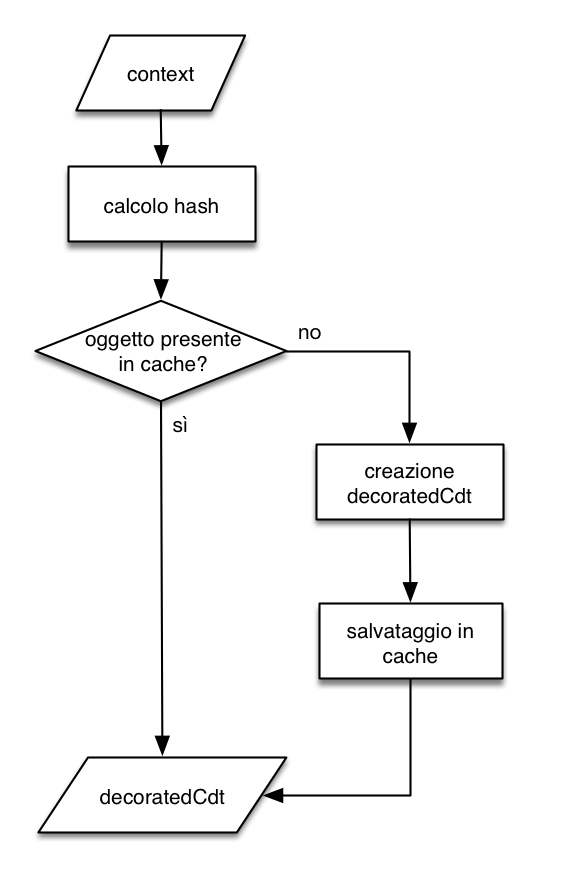
\includegraphics[width=0.43\textwidth]{4-progettazione-alto-livello/Immagini/diagramma_flusso_decoratedCdt.png}
	\caption{Flusso di creazione del CDT decorato\label{fig:flusso-decorated-cdt}}
\end{figure}

\subsubsection*{Acquisizione dei dati primari}

\begin{figure}[!t]
	\centering
	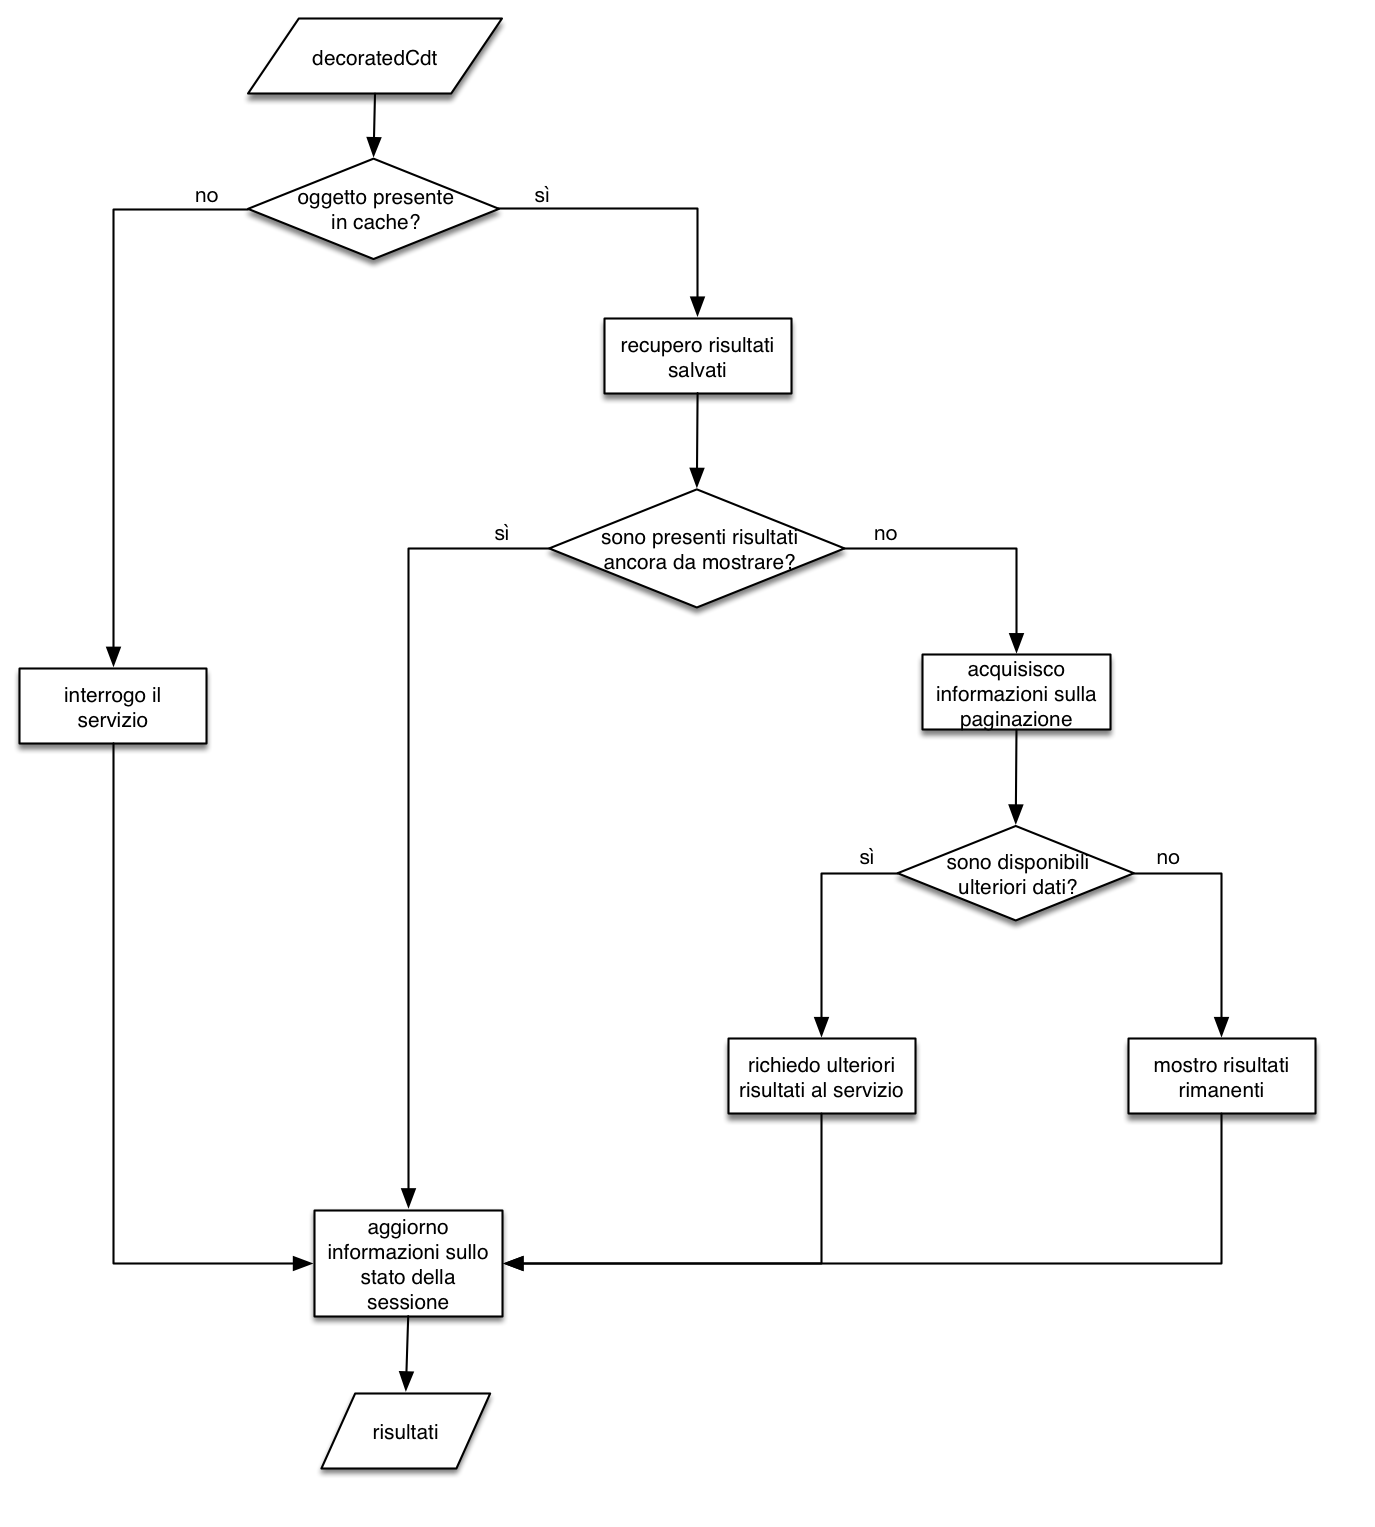
\includegraphics[width=\textwidth]{4-progettazione-alto-livello/Immagini/diagramma_flusso_servizi_primari.png}
	\caption{Flusso di richiesta dei risultati primari\label{fig:flusso-servizi-primari}}
\end{figure}

Questa fase viene eseguita una volta terminata la creazione del \emph{CDT decorato}. In Figura \ref{fig:flusso-servizi-primari} viene mostrato il diagramma di flusso che mostra come viene gestita una richiesta.

La prima attività che viene svolta riguarda il controllo, come nel passaggio precedente, se la richiesta era già stata gestita in passato. Se si tratta di una nuova richiesta, l'attività viene svolta dai componenti che fanno parte del blocco \virgolette{Primary Service} nella Figura \ref{fig:flusso-nuova-richiesta}. Il primo componente che viene eseguito è il \emph{Primary Service Selection}, che si occupa di selezionare le operazioni che sono più idonee al contesto fornito dall'utente. Prodotto l'elenco entra in gioco il \emph{Query Handler}, che ha un duplice compito: il primo, con l'ausilio di uno o più \emph{Bridge}, è l'invocazione dei servizi prescelti mentre il secondo è l'acquisizione delle relative risposte. Una volta ricevute le risposte provvede a trasformarle nel formato interno, tramite le funzioni messe a disposizione dal \emph{Response Parser}. Tutte le risposte ricevute vengono infine unite a formare un'unica lista e restituite per essere ulteriormente elaborate dal \emph{Response Aggregator}, che effettua un'attività di rimozione dei duplicati. L'elenco dei risultati identificato verrà dunque salvato per un periodo di tempo in cache in modo da poter essere riutilizzato per richieste future.

L'altra eventualità si verifica quando la risposta è presente in cache. Questo caso ha una gestione un po' più complessa rispetto al precedente perché viene considerata anche la paginazione dei risultati. La prima verifica riguarda la disponibilità di informazioni da restituire al client. Se la quantità di dati contenuti in cache è sufficiente a evadere la richiesta viene subito restituita la porzione di informazioni richiesta. Altrimenti viene effettuata una nuova richiesta verso i servizi che hanno ulteriori dati da mostrare. La regola di ricaricamento dei dati è la stessa descritta nella Sezione \ref{sec:session-helper}. Qualsiasi casistica termina sempre con l'aggiornamento dello stato nella cache, in quanto vengono sia salvati l'elenco dei risultati sia il numero di elementi che il client ha già richiesto. Il processo termina una volta che tutti i servizi non ha più dati da mostrare. In quel caso il client verrà informato del fatto che non sono più disponibili ulteriori pagine.

\subsubsection*{Acquisizione dei servizi di supporto}

Questa attività incomincia una volta creato il \emph{CDT decorato} e opera parallelamente all'acquisizione dei servizi primari. Coinvolge unicamente il componente \emph{Support Service Selection}, che si occupa di selezionare i servizi di supporto o gli intent richiesti dal client. In ingresso viene fornita la \emph{categoria} dei servizi che si vuole selezionare in base al contesto fornito.

Una volta selezionati incomincia la fase di composizione degli URL necessarie per interrogare il servizio o richiamare l'intent specifico.

\subsection{Mobile app}

In questa sezione si vuole analizzare il flusso dei dati all'interno dell'applicazione, partendo dal login dell'utente fino alla selezione di un elemento dalla lista dei risultati.

\begin{figure}[H]
	\centering
	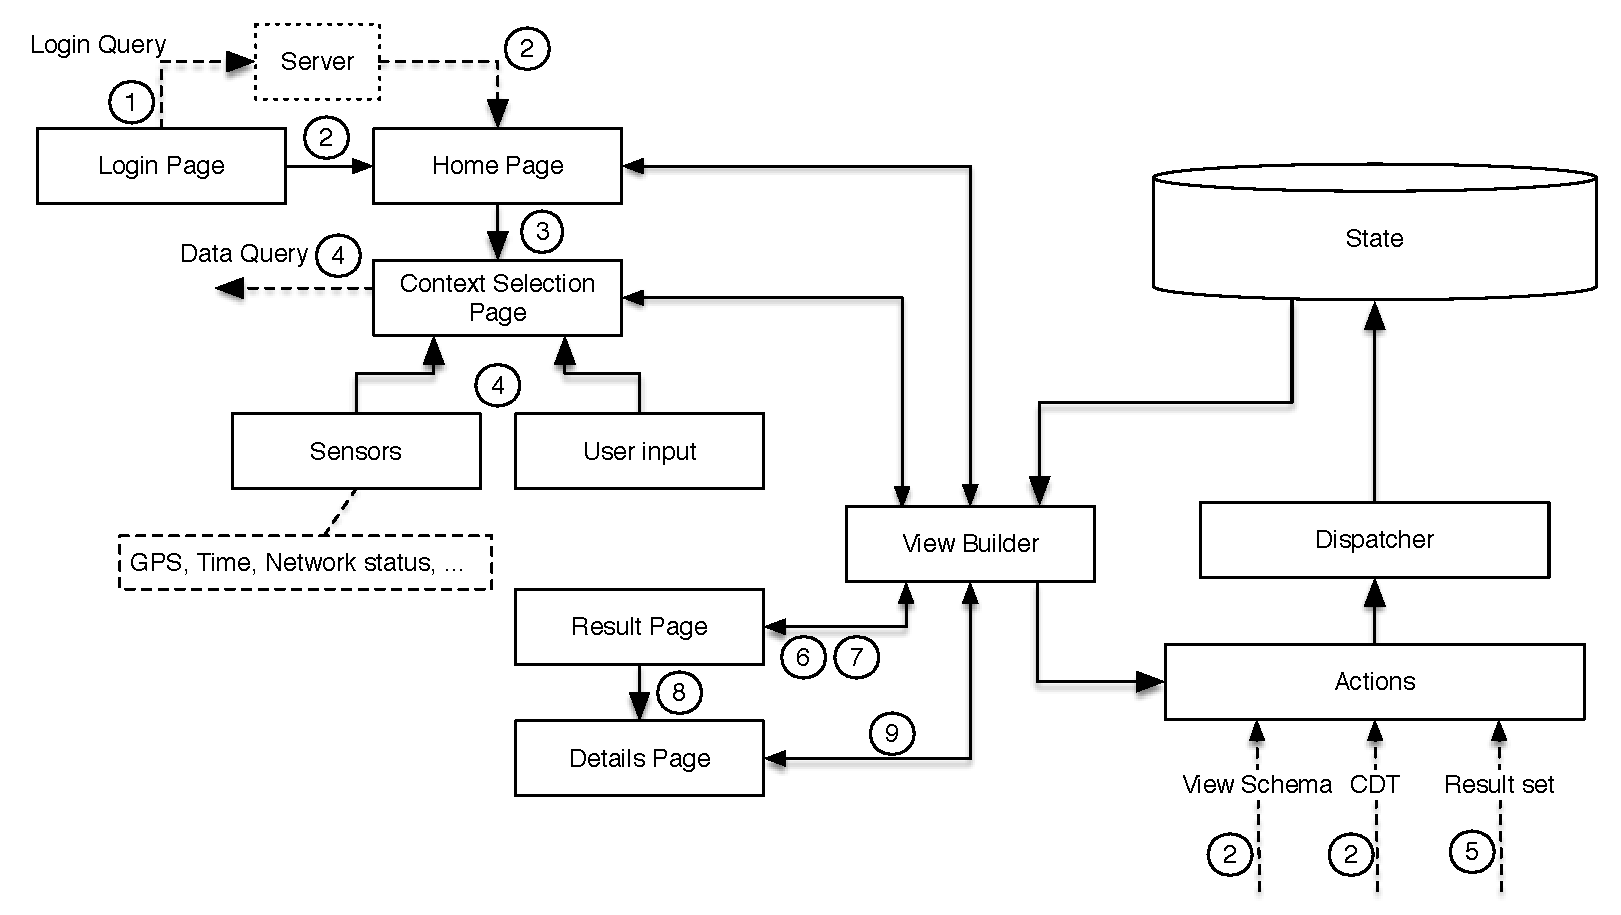
\includegraphics[width=\textwidth]{4-progettazione-alto-livello/Immagini/app_dataflow.pdf}
	\caption{Flusso dei dati dell'app Flux}\label{fig:app-dataflow}
\end{figure}

Nella Figura \ref{fig:app-dataflow} è rappresentato tutto il flusso dei dati all'interno dell'ap\-pli\-ca\-zio\-ne e di seguito vengono esposti i passaggi principali:

\begin{enumerate}
	\item
	La prima schermata che appare nell'applicazione è quella di login; qui l'utente inserisce le proprie credenziali e viene effettuata la richiesta GraphQL di login come definito in \ref{sec:login-endpoint}
	\item
	L'app riceve il CDT e i mashup dal server e quindi l'applicazione possiede tutto ciò che è necessario per caricare l'interfaccia grafica. Nel frattempo viene mostrata la pagina iniziale dell'applicazione
	\item
	L'utente seleziona l'\emph{Interest Topic} desiderato e viene reindirizzato alla pagina di selezione del contesto dove vengono mostrati i campi che devono essere compilati
	\item
	Dopo aver definito i parametri del contesto desiderati l'utente preme il bottone per effettuare la richiesta al server: l'applicazione recupera i dati inseriti dall'utente e allo stesso tempo i dati di posizione provenienti dai sensori del dispositivo mobile
	\item
	I dati di contesto sono composti assieme ai dati provenienti dai mashup per costruire la query GraphQL, come spiegato nella sezione \ref{sec:data-query}
	\item
	Il router dell'applicazione mostra all'utente la pagina dei risultati, la quale durante l'attesa della risposta dal server, continua a mostrare un'interfaccia di caricamento
	\item
	I risultati vengono processati insieme ai file di mashup per mostrare i dati nella pagina che mostra la lista di risultati
	\item
	L'utente scorre il result set ottenuto fino a quando non sceglie un elemento per visualizzarne i dettagli
	\item
	L'applicazione carica la pagina dove vengono visualizzati i dati completi relativi al dettaglio dell'e\-le\-men\-to selezionato e visualizzati nella pagina
\end{enumerate}

\section{Esempio del flusso di esecuzione}

\textcolor{red}{Completare ...}